\section{Methodology}

The methodology for predicting house prices involves the integration of data preprocessing, feature engineering, and model training. This section outlines the steps followed to build and evaluate the predictive model.

\subsection{Data Preparation}
The dataset is compiled from three primary sources: MLS Home Price Index (HPI), Consumer Price Index (CPI), and Canada Prime Rate. These indicators, recorded at different frequencies, are unified through resampling and interpolation to ensure consistency:
\begin{itemize}
    \item Monthly CPI data is interpolated to a daily frequency.
    \item Prime rate data, initially provided at discrete time points, is also resampled to daily intervals.
    \item HPI data, sourced from multiple regional Excel sheets, is interpolated for missing values and merged into a single dataset.
\end{itemize}

\subsection{Feature Engineering}
To prepare the data for modeling:
\begin{itemize}
    \item \textbf{Dimensionality Reduction:} Highly correlated features (with a correlation coefficient $>$ 0.6) relative to the target variable, the Single-Family HPI, are removed to avoid multicollinearity.
    \item \textbf{Normalization:} Standard scaling is applied to all features, ensuring zero mean and unit variance for improved model convergence.
    \item \textbf{Dataset Splits:} The data is divided into training (70\%), validation (10\%), and testing (20\%) sets to ensure robust model evaluation.
\end{itemize}

\subsection{Model Training}
The training process involves:
\begin{itemize}
    \item \textbf{Loss Function:} A weighted combination of Mean Squared Error (MSE) for prediction and reconstruction loss for auxiliary supervision ensures the model learns to accurately predict while preserving key data patterns.
    \item \textbf{Optimizer:} The Adam optimizer is used with gradient clipping to stabilize training and prevent exploding gradients.
    \item \textbf{Hyperparameters:} Model parameters, such as the learning rate, number of LSTM layers, and latent space dimensions, are fine-tuned to optimize performance.
\end{itemize}

\subsection{Evaluation Metrics}
The model is evaluated using:
\begin{itemize}
    \item \textbf{Mean Squared Error (MSE):} Quantifies prediction accuracy by measuring the average squared difference between actual and predicted values.
    \item \textbf{R² Score:} Assesses the proportion of variance in the target variable explained by the model.
\end{itemize}

\subsection{Implementation and Logging}
The model is implemented in PyTorch, with:
\begin{itemize}
    \item \textbf{Data Loaders:} Efficiently handling the training, validation, and test datasets.
    \item \textbf{MLflow Integration:} Logging model parameters, training losses, validation scores, and final test results to ensure reproducibility and facilitate future experimentation.
    
    \item \textbf{Visualization:} Key training metrics and model performance are visualized using Matplotlib and logged with MLflow for easy tracking and comparison.
    
    \begin{figure}[H]
        \centering
        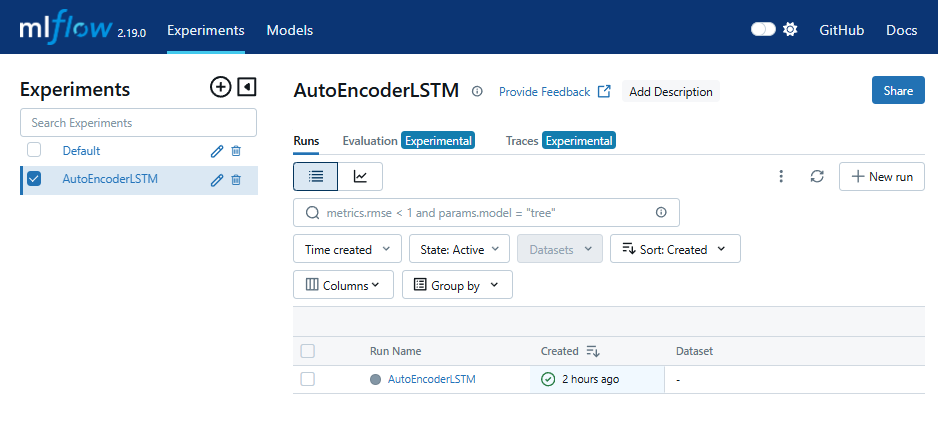
\includegraphics[width=0.8\textwidth]{images/mlflow.png}
        \caption{MLflow logging and visualization of model training metrics.}
        \label{fig:mlflow}
    \end{figure}
\end{itemize}
\subsection{Folder Structure Overview}
The folder structure for the project is organized to ensure clarity, modularity, and ease of maintenance. Below is a detailed explanation of each directory and its contents:

\begin{itemize}
    \item \textbf{.conda Directory:} This directory contains configuration files and dependencies managed by the Conda environment. It ensures reproducibility of the Python environment used for the project.
    
    \item \textbf{data Directory:} This folder contains all the raw datasets required for the project:
    \begin{itemize}
        \item \texttt{CPI\_MONTHLY.csv}: Contains Consumer Price Index (CPI) data, which measures inflation trends.
        \item \texttt{house\_price\_index.xlsx}: Contains MLS Home Price Index (HPI) data for different regions in Canada.
        \item \texttt{Prime-Rate-History.csv}: Includes historical data on Canada's prime interest \\rates.
    \end{itemize}
    Additionally, a subfolder named \texttt{dataloader} is used to store pickled versions of preprocessed data loaders, facilitating quick access to training, validation, and testing datasets.
    
    \item \textbf{mlartifacts and mlruns Directories:} These directories are part of the MLflow tracking system. They store logged model artifacts, parameters, metrics, and experiment run details. MLflow ensures reproducibility and traceability of the model development process.
    
    \item \textbf{model Directory:} This directory contains all files related to the definition and training of the Autoencoder-LSTM model:
    \begin{itemize}
        \item \texttt{\_\_init\_\_.py}: Initializes the model module.
        \item \texttt{model.py}: Defines the architecture of the Autoencoder-LSTM model.
        \item \texttt{params.json}: Stores hyperparameters such as input dimensions, learning rates, and the number of LSTM layers.
        \item \texttt{utils.py}: Includes helper functions for training and evaluation of the model.
    \end{itemize}
    
    \item \textbf{preprocessing Directory:} This directory houses the preprocessing scripts:
    \begin{itemize}
        \item \texttt{load\_cpi.py}: Processes the CPI data, including interpolation and merging of historical revisions.
        \item \texttt{load\_hpi.py}: Handles the HPI data by reading multiple Excel sheets, performing linear interpolation, and merging them into a single dataset.
        \item \texttt{load\_rate.py}: Prepares the prime rate data by resampling and interpolating missing values.
        \item \texttt{\_\_init\_\_.py}: Initializes the preprocessing module.
    \end{itemize}
    
    \item \textbf{report Directory:} This directory is used to store the project's documentation, including the final report and visualizations generated during the project.
\end{itemize}

\textbf{Root-Level Files}
\begin{itemize}
    \item \texttt{main.py}: The main script orchestrates the entire workflow, including data preprocessing, model training, and evaluation. It integrates modules from the preprocessing and model directories.
    \item \texttt{requirements.yml}: Specifies the dependencies and environment configurations required to replicate the project.
    \item \texttt{.gitignore}: Lists files and folders to be excluded from version control.
\end{itemize}

By combining careful data preparation, feature engineering, and the hybrid Autoencoder-LSTM model, this methodology achieves robust and accurate predictions of house prices, addressing both the high dimensionality and sequential characteristics of the dataset.